
\documentclass[11pt, openany]{report}
\usepackage{euler}
\usepackage{amsmath}
\usepackage[utf8]{inputenc}
\usepackage[linesnumbered,ruled,vlined]{algorithm2e}
\usepackage[OT1]{fontenc}
\usepackage[a4paper,left=2cm,right=2cm,top=2cm,bottom=2cm]{geometry}
\usepackage[frenchb]{babel}
\usepackage{libertine}
\usepackage[pdftex]{graphicx}
\usepackage{lmodern}
\usepackage{graphicx}
\usepackage{float}
\usepackage[export]{adjustbox}
\setlength{\parindent}{0cm}
\setlength{\parskip}{1ex plus 0.5ex minus 0.2ex}
\newcommand{\hsp}{\hspace{20pt}}
\newcommand{\HRule}{\rule{\linewidth}{0.5mm}}
\SetKwFor{For}{pour}{faire}{endfor}
\SetKwFor{While}{tant que}{faire}{endw}
\SetKwIF{If}{ElseIf}{Else}{si}{alors}{else si}{sinon}{endif}
\setlength{\parindent}{2em}
\setlength{\parskip}{0.2em}
\usepackage{titlesec}
\usepackage[nottoc,notlof,notlot]{tocbibind}
\titleformat{\section}{\bfseries\Large}{\thesection.}{0.5em}{}
\titleformat{\subsubsection}{}{\thesubsubsection}{1em}{\itshape}
\renewcommand\bibname{References}
\usepackage{glossaries}
\makeglossaries
\usepackage[%
	colorlinks=true,
	pdfborder={0,0,0},
	linkcolor=blue
]{hyperref}
\usepackage{fancyhdr}
\setlength{\headheight}{8pt}
\pagestyle{headings}
\renewcommand{\baselinestretch}{1}
\rfoot{Page \thepage}
\normalfont
\setlength{\parskip}{0.5em}
\begin{document}
\begin{titlepage}
  \begin{sffamily}
  \begin{center}
    % Upper part of the page. The '~' is needed because \\
    % only works if a paragraph has started.
    % \includegraphics[scale=0.04]{}~\\[1.5cm]


\begin{figure}[h!]
  \begin{minipage}{0.48\textwidth}
   \centering
  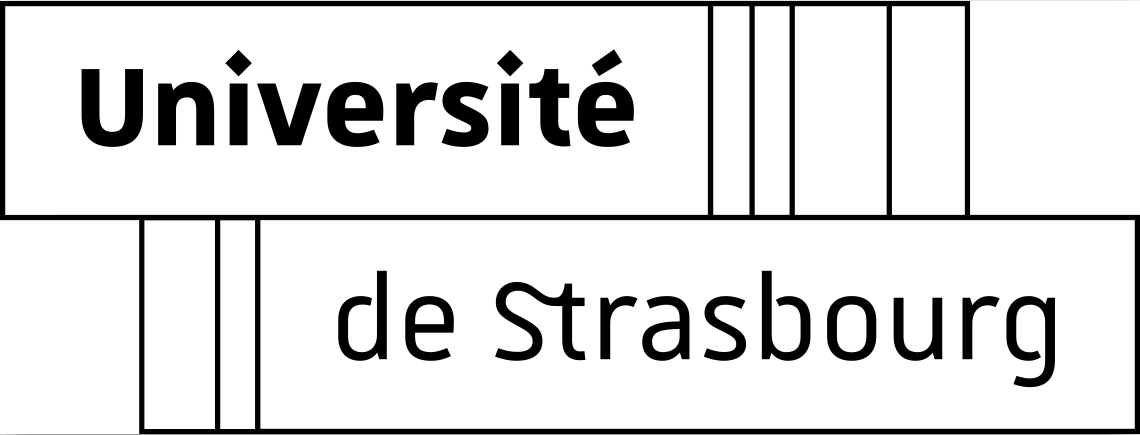
\includegraphics[width=0.6\linewidth,left]{unistra.png}
  \end{minipage}\hfill
  \begin{minipage}{0.48\textwidth}
   \centering
  
\includegraphics[width=0.6\linewidth,right]{eost.png}
  \end{minipage}
\end{figure}


    \textsc{\LARGE \\
Université de Strasbourg}\\[3cm]

    \textsc{\Large Rapport du Travail d'Etude et de Recherche}\\[1.5cm]

    % Title
    \HRule \\[0.4cm]
    { \Huge \bfseries
Validation de l’approche \\ clustering sous contraintes \\[0.4cm] }

\HRule \\[2cm]
	  	
    % Author and supervisor
    \begin{minipage}{0.4\textwidth}
      \begin{flushleft} \large
      	\textsc{Etudiant :}\\ 
        \textsc{Pambou Moubogha Eddy}\\
         \textsc{année scolaire 2019-2020}\\
      \end{flushleft}
    \end{minipage}
    \begin{minipage}{0.4\textwidth}
      \begin{flushright} \large
        \textsc{Encadrants :}\\ 
        \textsc{P. Gançarski}\\
        \textsc{A. Braud}\\
      \end{flushright}
    \end{minipage}

    \vfill

    % Bottom of the page
    {\large 1\ier{} Janvier 2020 — 12 Mai 2020}

  \end{center}
  \end{sffamily}
\end{titlepage}
\newpage
\tableofcontents

\chapter{Introduction}
Les glissements de terrain apparaissent lorsqu'une masse de terre descend sur un plan de glissement, provoqués par les activités anthropiques ou des phénomènes climatiques, géologiques ou géomorphologiques.
Ces déplacements peuvent être lents (quelques millimètres par an) ou rapides (quelques centaines de mètres par jour). \par

Ces mouvements peuvent être à l'origine de catastrophes naturelles causant des pertes humaines et des dommages importants sur les infrastructures. Au plan mondial, les mouvements de terrain causent chaque année la mort de 800 à 1000 personnes. En France, ce risque concerne environ 7000 communes et présente, pour un tiers d’entre elles, un niveau de gravité fort.\par

Bien que la détection de ces phénomènes soit difficile, il est possible de surveiller les mouvements du sol dans les zones sensibles en utilisant les techniques de télédétection. L'interférométrie radar et l'imagerie optique sont deux techniques de télédétection qui permettent de mésurer les mouvements du sol. L'interférométrie radar et l'imagerie optique. L'interférométrie radar est une technique de télédetection qui permet de mésurer la déformation du sol dans la ligne de visée du satellite avec une précision millimétrique en calculant la différence de phase entre deux acquisitions. Cependant, cette technique n'est pas adaptée pour mésurer les déplacements rapides. De plus, la déformation mésurée est une projection du vecteur déformation sur la ligne de visée du satellite, ne facilitant pas ainsi son interprétation. Contrairement à l'imagerie radar, l'imagerie optique permet de mésurer les déplacements rapides et est sensible aux composantes Nord-Sud et Est-Ouest de la déformation.

Il existe plusieurs algorithmes de correlation d'images. Des chercheurs de l'EOST travaillant au sein de l'équipe Déformation Active ont récemment proposé une nouvelle version de MPIC-OPT, un workflow permettant de calculer des champs de déplacement en utilisant la corrélation d'images. Cette nouvelle approche utilise la décomposition en composantes indépendantes (ICA) pour débruiter les déplacements bruts. Cependant, cette méthode statistique nécessite des heuristiques pour identifier les sources contribuant aux signaux d'interêt. Actuellement, cette étape n'est pas automatique, et est réalisée en utilisant les connaissances sur la zone d'étude.\par

Dans un premier temps, est de propose d'automatiser la détection de glissements de terrain en utilisant les techniques de machine learning. Dans un second temps, il vise à dévélopper une approche pour fusionner les données de l'imagerie radar et de l'imagerie optique afin d'avoir une meilleure cartographie des glissements de terrain.

\chapter{Présentation de l'organisme d'accueil}
L'Ecole et Observatoire des Sciences de la Terre (EOST) est une école d'ingénieurs en géophysique
créé en 1935 par Edmond Rothé. Comme son nom l'indique l'EOST est également un observatoire. L’objectif premier de l’UMS830 est de faciliter l'observation pérenne des phénomènes naturels et de rendre accessible les données recueillies à la communauté scientifique. Ses tâches d'observation entrent dans le cadre des Services Nationaux d'Observation (SNO) labellisés par l'Institut National des Sciences de l'Univers du CNRS. Au total, l'EOST est impliqué dans dix services d'observation dont il est pilote au plan national ou partenaire actif. Ils concernent le domaine "Terre solide" et le domaine "Surfaces et interfaces continentales".

Ce stage s'effectue au sein de l'équipe Déformation Active. Les travaux de l'équipe portent sur la déformation lithosphérique, le fonctionnement des failles sismiques et la déformation de sub-surface. Elle est fédérée autour de plusieurs disciplines, telles que la géodésie, la tectonique active, la géomorphologie et la paléosismologie. Elle appuie fortement sa recherche sur les données acquises par les observatoires de l'EOST gérés par ses membres et sur des chantiers régionaux, principalement situés en Méditerranée et en Afrique.

\chapter{Méthodes}
\chapter{Résultats}



\section{Contraintes}


Lorsque les données sont labellisées, les contraintes Must-Link et Cannot-Link se déduisent aisement .
Dans la pratique , les données labellisées sont difficiles à obtenir (trop couteux) . En l'absence de telles données ,  les contraintes peuvent etre neanmoins rajoutées en se basant uniquement sur des connaissances . Les contraintes sont donc plus générales que les étiquettes .
\newpage
On peut citer d'autres contraintes parmi lesquelles :
\begin{itemize}
  \item le nombre de cluster  ; 
   \item le diamètre maximum : les clusters doivent avoir un diamètre maximum de $\gamma$ ;
    \item  le $\epsilon$ - voisinage  :  un objet doit avoir au moins un voisin dans un rayon de $\epsilon$ ;
     \item la séparation : les clusters doivent au moins être distants de $\delta$ .
\end{itemize}

\begin{figure}[h!]
  \centering
  \caption{Example de contraintes ML , CL , $\gamma$ , $\delta$ et $\epsilon$}
  \label{fig:contraintes}
\end{figure}

\chapter{Les méthodes de partitionnement} 
\section{K-means}

\section{SAMARAH}

La phase (2)  se compose de 4 sous-phases :

\begin{enumerate}
 \item  détection des conflits  en évaluant les dissimilarités entre les pairs de résultats  ;
  \item le choix des conflits à résoudre ;
   \item la résolution locale des conflits ;
    \item l'integration des modifications locales dans le résultat global .
\end{enumerate}


\subsubsection{Modifications et convergence des résultats}
\setlength{\parindent}{0in}
Pour faire converger les résultats des clustering , il faut une méthode qui permet de mésurer la similarité entre deux clusters . Elle ne repose pas sur une distance  puisque le calcul d'une distance entre deux objets n'est pas toujours possible . Pour une classe $C_{k}^i$ appartenant au résultat $R_i$, sa classe correspondante  dans le resultat $R^j$ est la classe $C_{k_m}^j$ avec laquelle il a le plus d'objets en commun .

Pour calculer la similarité entre la classe $C_{k_m}^i$ et sa classe correspondante, il faut connaitre :

\begin{itemize}
  \item la distribution de la classe $C_k^i$ dans le résultat $R^j$ :
  \[
  		\rho_k^{i,j} = \sum_{l=1}^{n_j} \left( \alpha_{k,l}^{i,j} \right)^2 \mathit{avec}  \alpha_{k,l}^{i,j} = \frac{|C_k^i \cap C_l^i|}{|C_k^i|}
  	\]
   \item la proportion d'objets de la classe $C_k^i$ dans le résultat $R^j$  :
    \[  		
    	\alpha_{{k_m},k}^{j,i} = \frac{|C_{k_m}^j \cap C_k^i|}{|C_{k_m}^j|}
  	\]
\end{itemize}

\subsubsection{Combinaison des résultats}
\setlength{\parindent}{0in} 
Quand il n'y a plus de conflits à résoudre , les résultats de chaque classifieur sont très similaires.
On distingue deux cas : 

\begin{itemize}
	\item les résultats ont tous le même nombre de clusters  : on peut alors associer à chaque cluster d'un résultat $R^i$ , le cluster qui lui correspond dans le résultat $R^j$  de manière unique  et appliquer un alorgorithme de vote ;
	\item la condition précédente n'est pas vérifiée : une nouvelle méthode de vote est définie .\\
\end{itemize}
Lorsque les résultats n'ont pas tous le même nombre de classes , on s'interesse aux groupes consensuels et aux objets non consensuels .
Un groupe d'objets consensuels est un ensemble d'objets appartenant au même cluster et qui sont classés de la même manière dans la majorité des résultats (un tel groupe est peut-être une forme forte) . \par
Un objet non consensuel est un objet qui n'appartient pas à un groupe consensuel . Ces objets correspondent souvent à ceux les plus éloignés du centre d'un cluster .
\newline
En resumé , la solution unifiée est composée des groupes consensuels auxquels on réaffecte les objets non consensuels (à l'aide des k-means par exemple ) .
\newline
\newline
\begin{algorithm}[H]
\textbf{procedure} SAMARAH(dataset $\mathcal{O}$ , ensemble d'agents $\mathcal{A}$ , contraintes must-link ML  $\subseteq$  $\mathcal{O}$   $\times$  $\mathcal{O}$ , contraintes cannot-link CL $\subseteq$  $\mathcal{O}$   $\times$  $\mathcal{O}$   )

  \For{chaque agent $a_i$ de $\mathcal{A}$ }    
        { 
        	partitionner  $\mathcal{O}$ en utilisant $a_i$
        }
  Créer l'ensemble des conflits  $\mathcal{C}$ en evaluant les dissimilarités entre les pairs de resultats \\
  Soit $\mathcal{E}$ l'évaluation des résultats initiaux en fonction du critère de collaboration\\
   \While{ $\mathcal{C}$ est non vide }
   {
   		choisir un conflit à résoudre de $\mathcal{C}$ \\
   		effectuer une résolution locale avec les agents impliqués \\
   		Soit $\mathcal{E}'$ l'évaluation des nouveaux resultats en fonction du critère de collaboration \\
   		\If{ $\mathcal{E'}  >  \mathcal{E}$  }
    	{
       		$\mathcal{E'}  =  \mathcal{E}$ \\
       		appliquer les modifications aux agents \\
       		calculer le nouvel ensemble de conflits \\
       		supprimer les conflits non résolus \\
   		}
   		
   		
   }
 
 calculer la  solution unifiée en utilisant un algorithme de vote
\caption{SAMARAH}
\end{algorithm}







\chapter{Validation}
Dans ce chapitre , nous exposerons premièrement les approches utilisées pour valider les résultats d’un algorithme de classification . Ensuite , nous présenterons  quelques  indices qui nous permettent d'implémenter la validation .  

\section{Méthodes de validation}
La notion de cluster est difficile à définir . Elle dépend de l’objectif à atteindre et nécessite une bonne connaissance des données .  Il existe deux approches permettant de valider les résultats d’un algorithme d’apprentissage : la validation interne et externe . A ces deux approches ,
nous rajouterons une étude de la stabilité de l'algorithme .
\subsection{Validation interne}
On parle de validation interne lorsque les résultats d’un clustering sont évalués par rapport à eux-mêmes . La validation interne est réalisée à l'aide de critères de qualité dit \emph{internes} . Ces critères permettent de mesurer la compacité et la séparabilité des clusters .

Dans cette étude , plusieurs critères semblent peu pertinents . Il s'agit notamment de l'inertie  et des indices de Dunn et Davies-Bouldin . La difficulté à utiliser ces indices provient du fait que Samarah ne renvoie pas toujours un résultat avec le même nombre de clusters pour une configuration de départ donnée . Comme le nombre de clusters en sortie varie , moyenner les résultats  n'est pas approprié . Pour évaluer la qualité interne d'un clustering , nous utiliserons plutôt une approche \emph{objet bien classé} et \emph{objet mal classé} .\par
Pour quantifier l'homogénéité et la séparation d'un clustering , on peut mesurer ce que l'on appelle le coefficient de silhouette . Pour un point $x$ donné, le coefficient de silhouette $s(x)$ permet d'évaluer  si ce point est proche des points  du cluster auquel il appartient (homogénéité)  et  loin des autres autres points(séparation) .
\newline
\newline
\newline
\newline

Pour quantifier l'homogénéité ,  on calcule la distance moyenne de $x$ à tous les autres points du cluster $C_k$ auquel il appartient : 
\[
	\mathit{a(x)} = \frac{1}{ |C_k| - 1 }\sum_{ u \in C_k , u \not\in x}d(u,x)
\]
Pour quantifier la séparation , on calcule la plus petite valeur que pourrait prendre a(x), si x était assigné à un autre cluster :
\[	
	\mathit{b(x)} =  min_{\mathit{ l \neq l } } \frac{1}{|C_l|} \sum_{u \in C_l}d(u,x) 
\]
 Si $x$ a été correctement assigné, alors $a(x) < b(x)$. Le coefficient de silhouette est donné par :
\[	
	\mathit{s(x)} = \frac{ a(x) - b(x) }{ max ( a(x) , b(x) )} 
\]
Il est  compris entre -1 et 1, et d'autant plus proche de 1 que l'assignation de $x$ à son cluster est satisfaisante . Pour évaluer la qualité interne globale , on calcule coefficient de silhouette moyen.

\subsection{Validation externe}
On parle de validation externe lorsque les résultats d’un clustering sont évalués à l'aide de connaissances extérieures . Elle est réalisée à l'aide de critères de qualité dit \emph{externes} . De manière générale , ils permettent de comparer deux partitions  : l'une est le résultat d'un algorithme de classification et l'autre est une vérité-terrain (les deux partitions peuvent avoir un nombre de clusters différent) . Il existe plusieurs indices externes , nous présentons ici ceux choisis pour notre étude .

Soit deux partitions $\pi_1$  et $\pi_2$ , et soient les comptages suivantes :
\begin{itemize}
  \item $sd$ : le nombre de couple d'objets dans le même cluster dans la partition $\pi_1$ ;
   \item $dd$ : le nombre  de couples d'objets differents dans les deux partitions ;
    \item $ds$ : le nombre de couple d'objets dans le même cluster dans la partition $\pi_2$ ;
     \item $ss$ : le nombre de couples d'objets dans le même cluster dan les deux classes ;
     \item $mm$ : le nombre total de couple d'objets . \\
\end{itemize}
Le critère de similarité de Jaccard est donnée par :
\[
	J(\pi_1 , \pi_2 )= \frac{|\pi_1 \cap \pi_2|}{|\pi_1 \cup \pi_2|} = \frac{ss}{ss + sd + ds} \in \lbrack 0 , 1 \rbrack
\]
Le critère de qualité de Folkes-Mallows est  donnée par :
\[
	FM(\pi_1 , \pi_2 ) = \sqrt{ \left( \frac{ss}{ss + sd} \right) \left(\frac{ss}{ss + ds} \right) } 
\]
L'indice de Hubert  permet de mésurer la corrélation entre deux matrices \cite{R} . Lorsque les matrices sont symétriques , il se definit par  :

\[
	\bar{\Gamma}(P,Q) = \frac {\sum_{i=0 ,i < j}^{n-1}\left(P_{ij} - \mu_P \right)\left(Q_{ij} - \mu_Q \right)}{\sigma_P\sigma_Q}  \in \lbrack -1 , 1 \rbrack 
\]

Où 
$P$ est la matrice de proximité du jeu de données  ,
$Q$ est une matrice $n \times n$ où $(i,j)$ represente la distance entre les centres des clusters auxquels  les objets $O_i$ et $O_j$ appartiennent ,
$\mu_P$, $\mu_Q$, $\sigma_P$, $\sigma_Q$ sont respectivement  les moyennes et les variances des matrices $P$ et $Q$ . 

En apprentissage semi-supervisée , la validation externe est par définition impossible à réaliser puisqu'on ne dispose pas de données etiquetées . Les indices choisis nous permettront d'étudier la stabilité  de l'algorithme .

\section{Stabilité des clusters}
Le résultat d'un algorithme de classification dépend de ses paramètres et  des données sur lequel il est appliqué . On dit qu'il est stable si de legères variations dans les données ou  des initialisations différentes n'induisent pas de grandes variations en sortie  . L'idée est que s'il existe un nombre de clusters $n$  correspondant à la structure naturelle des données (en excluant les cas triviaux),  plusieurs exécutions de l'algorithme avec $n$ clusters et des paramètres differents doivent conduire à des partitions très similaires . De ce fait , ce principe peut être utilisé pour trouver le nombre optimal de clusters .

\chapter{Application}
\section{Jeux de données }
Les jeux de données proviennent de la base de données du projet ANR FRESQAU . Chaque jeu de données est composé d'un ensemble de stations identifiés par des numéros . Chaque station mésure la concentration  de  divers éléments chimiques ou biochimiques renseignant sur la qualité de l'eau .

\begin{figure}[H]
  \centering
  \caption{Exemple de données collectées par la station 402123 (premières lignes) .}
  \label{fig:contraintes}
\end{figure}

\section{Méthodologie}
Deux jeux de données de la base de donnees issue du  projet FRESQAU  ont été choisis pour réaliser nos experiences . Elles comportent moins de 50 \%  de valeurs manquantes .  Les données de base sont transformées et stockées suivant le mode séquentiel  . En mode séquentiel , les valeurs manquantes des données de base sont ignorées dans le format final des données .

Dans la configuration de Samarah ,  il est possible de spécifier le nombre de clusters mininum et le nombre de clusters maximum (il s'agit d'une contrainte sur le nombre de clusters) . Cela signifie qu'on souhaite obtenir un résultat dont le nombre de clusters est situé entre ces deux bornes . Cette contrainte est interessante si elle est suggerée par un expert . Dans notre cas ,  il apparait très peu pertinent de vouloir imposer une contrainte sur le nombre de cluster alors que c'est l'inconnue que l'on cherche à déterminer . Le nombre de cluster minimum a donc été fixé à 2 et le nombre de cluster maximum à 20 pour tous les tests .

Le nombre de clusters varie entre 2 et  20 . Nous avons choisi 2 agents k-means avec le même nombre de clusters . Pour étudier la stabilité de l'algorithme sur les données , nous avons exécuté  SAMARAH  10 fois pour un nombre de cluster fixé .\par Les critères de qualité de  Hubbert,  Jaccard , Folkes-Mallows , Wemmert obtenus pendant les tests sont moyennés (Ces critères sont déjà implémentés dans Multicube) .

Pour évaluer la qualité interne d'une partition , nous avons choisi le coefficient de silhouette . Il est borné  et donc plus facile à intepréter . Toutefois pour s'assurer de la fiabilité des résultats obtenus , nous avons défini un critère de qualité  $\Delta$ . $\Delta$ est une moyenne des écarts entre le nombre  de clusters en entrée et le nombre de nombre de clusters en sortie . S'il est proche  de 0  alors le nombre de clusters en entrée a été égale au nombre de clusters en sortie . Plus généralement ,  une faible valeur indique une faible variabilité des résultats en terme de nombre de clusters .

Pour évaluer le comportement de l'algorithme en fonction de la consistence des contraintes,  deux jeux de contraintes sont crées à partir des resultats de Samarah : un jeu de contraintes \emph{consistentes}(au sens de non aléatoire)  et un jeu de contraintes aléatoires . Pour créer une contrainte consistente , on choisi un objet aléatoirement  . On calcule son coefficient de silhouette  .  Si la valeur obtenue est inférieure à une valeur seuil $\gamma$   alors l'objet est considéré mal classé . Dans ce cas ,  on crée une contrainte Cannot-Link entre cet objet et un objet quelconque appartenant au même cluster . Si la valeur obtenue est supérieure à $\gamma$ , l'objet est considéré bien classé . On crée alors une contrainte Must-Link entre cet objet et un objet quelconque appartenant au cluster dont il est le plus proche . Comme le coefficient de  silhouette varie entre -1 et 1 , la valeur la plus naturelle  de $\gamma$ semble être 0 .Cependant ,  quelques tests ont montré qu'il y a très peu d'objets dont le coefficient de silhouette est inferieure à 0 . De ce fait , fixer la valeur de $\gamma$ à 0 va plus favoriser la création de contraintes Must-Link . Pour éviter ce déséquilibre , nous avons choisi de fixer la valeur de $\gamma$ à 0.25 . Pour créer une contrainte  aléatoire , on choisit deux points au hasard  ; s'ils appartiennent au même cluster , on crée une contrainte Cannot-Link sinon on crée une contrainte Must-Link . La création d'une contrainte aléatoire ne depend pas de $\gamma$ .  Il n' y a aucune méthode pour mésurer la consistence d'un jeu de contraintes avec la distance élastique . Pour avoir un aperçu de l'utilité des contraintes ,  on calcule le ratio $\frac{DistML}{DistCL}$ . Le numérateur représente  la distance moyenne entre les pairs de contraintes Must-Link ; le dénominateur représente la distance moyenne  entre les pairs de contraintes Cannot-Link  . Si ce ratio est inférieure à 1 , cela signfie que les paires de contraintes Must-Link sont en moyenne plus proches  que les paires de contraintes Cannot-Link . Ce ratio a été  aussi utilisé pour bien s'assurer que les contraintes créées aléatoirement ne sont pas nécessairement \emph{consistentes} .

Pour chaque résultat de Samarah , nous avons relancé une itération avec le jeu de contraintes consistentes et le jeu de contraintes aléatoires . Les deux nouvelles partitions obtenues sont comparées en utilisant les indices de qualités retenues . Le pourcentage d'objets auxquels on assigne des contraintes a été fixé à 15\% .


\section{Résultats}
Les résultats  du jeu de données PHOSV2 obtenus sans contraintes montrent que tous les indices de similarité décroîssent quand le nombre de clusters augmente (Figure ~\ref{fig:criteriaEvolution}) .
On remarque que $\Delta$ varie très peu pour un nombre de cluster donné . On note de très faibles valeurs entre 2 et 4 clusters pour le jeu de données PHOSV2 . Dans l'ensemble , il croît  quand le nombre de clusters augmente . Il vaut en moyenne  0,98 pour 2  clusters . L'ajout des contraintes aléatoires et non aléatoires n'affecte pas le comportement des critères de similarité  (Figure ~\ref{fig:phosvNoEvolution}).
Sur le jeu NITRV1 , on note une décroissance rapide du coefficient de silhouette . La meilleure partition affiche une valeure inférieure à 0.4 (Figure ~\ref{fig:nitrvEvolution}).

\begin{figure}[H]
  \centering
  
\includegraphics[width=0.6\linewidth]{eost.png}
  \caption{Evolution des critères de similarité en fonction de nombre de classes pour le jeu de données PHOSV2 : en bleu les résultats obtenus avec les données standardisées , en rouge ceux obtenus avec les données normalisées .}
  \label{fig:criteriaEvolution}
\end{figure}

\begin{figure}[H]
  \centering
  \includegraphics[width=0.6\linewidth]{imageComparison.png}
  \caption{Evolution des critères de similarité après ajout de contraintes aléatoires et consistentes pour  le jeu de données PHOSV2 . Les courbes sont confondues car aucune contrainte n'a été violée .}
  \label{fig:phosvNoEvolution}
\end{figure}

\begin{figure}[H]
  \centering
  \includegraphics[width=0.6\linewidth]{contraintesEffect.png}
  \caption{Effet des contraintes aléatoires obtenu avec le jeu de données NITRV2 standardisées . Le pourcentage  de contraintes violées  est calculé après avoir relancé Samarah avec un jeu contraintes. }
  \label{fig:nitrvEvolution}
\end{figure}

\section{Discussion}
Dans cette partie ,  nous analyserons les résultats de nos tests en les mettant en relation avec le fonctionnemment de Samarah  et les connaissances générales sur le clustering .

\subsubsection{Sensibilité de l'algorithme}
\setlength{\parindent}{0in}
Les résultats montrent que l'algorithme est sensible à l'initialisation . Cette remarque s'explique par la faible variation de  $\Delta$  et à la croissance observée . Si par exemple , la structure des données contient 4 clusters , il est peu probable que l'algorithme  renvoie souvent 4 clusters si les agents ont un nombre de clusters très éloigné de ce dernier . Par conséquent , il est important d'imposer une contrainte sur le nombre de clusters minimum et maximum en se basant sur l'avis d'un expert .

\subsubsection{Qualité interne et nombre de clusters}
\setlength{\parindent}{0in}
La décroissance des critères de similarité quand le nombre de clusters augmente est un comportement évident . Le fait le plus marquant est la croissance de $\Delta$ . Les faibles variations de $\Delta$ pour un cluster donné peuvent s'expliquer par le fait que lorsque les agents ont au départ le même nombre de clusters ,  il y a plus de chance d'avoir des objets distribué de la même façon  et donc très peu de conflits à résoudre . On se retrouve très vite dans la configuration que Samarah essaie d'atteindre . En conséquence le nombre de clusters final aura tendance à osciller légèrement autour du nombre de cluster en entrée . Si cette hypothèse était vraie alors l'écart absolu mésuré serait relativement constant pour tous les tests . Or on remarque  que cet écart croît . Cette croissance provient donc du fait que l'algorithme devient de plus en instable lorsque qu'on s'éloigne du nombre de clusters optimal . Cette instabilité se traduit par une distribution aléatoire des objets d'où la décroissance du coefficient de silhouette qui montre que les objets sont de plus en plus mal classés (Figure ~\ref{fig:criteriaEvolution}) . 
\newline
\newline
A cause de la variabilité des résultats , on peut seulement affirmer que le nombre de clusters se situe entre  2 et 4 pour le jeu de données PHOSV2 et 2 pour NITRV2 (Figure ~\ref{fig:nitrvEvolution}) .

\subsubsection{Influence de la normalisation}
\setlength{\parindent}{0in}


\subsubsection{Influence de la cohérence des contraintes}
\setlength{\parindent}{0in}
Les tests effectués pour étudier le comportement de l'algorithme en fonction des contraintes ne sont pas concluants . Sur le jeu de données PHOSV2 , on ne note aucune différence après l'ajout des contraintes (Figure  ~\ref{fig:phosvNoEvolution}) . \\
Sur le jeu  de données NITRV2 réalisé avec un autre scénario de test (on a juste lancé samarah une fois au lieu de deux) , le ratio $\frac{DistML}{DistCL}$ est très élévé , ce qui implique que les paires de contraintes Cannot-Link sont plus proche en moyenne que les paires de contraintes Must-Link (c'est effectivement le cas par construction des contraintes aléatoires) . Aucune relation claire  entre la qualité des contraintes et le pourcentage de contraintes violées ne se dégage (Figure ~\ref{fig:nitrvEvolution}) .
\newline
\newline
\chapter{Conclusion}
\setlength{\parindent}{2em}



\newpage
\newpage
\begin{thebibliography}{9} 
\bibitem{UVL} Ulrike von Luxburg ,\emph{ Clustering stability : an overview} .

\bibitem{IBMDU}Ismail Bin Mohamad and Dauda Usman  ,\emph{ Standardization and Its Effects on K-Means Clustering Algorithm } .

\bibitem{NL}  Nicolas Labroche  ,\emph{ Méthodes d’apprentissage automatique pour l’analyse des interactions utilisateurs 
} .

\bibitem{TP}T. Lampert, T. Dao, B. Lafabregue, N. Serrette, G. Forestier, B. Crémilleux, C. Vrain, P. Gancarski  ,\emph{ Constrained distance based clustering for time-series: a comparative and experimental study} .

\bibitem{UVL}Kiri Lou Wagstaff   ,\emph{ Intelligent clustering with instance
level constraints} .

\bibitem{FP}F. Petitjean , A. Ketterlin, P. Gancarski   ,\emph{ A global averaging method for dynamic time warping,with applications to clustering } .

\bibitem{ASFXCNFM} A. Braud, S.  Bringay, F. Cernesson, X. Dolques, M. Fabrègue, C. Grac, N.  Lalande, F. Le Ber, M. Teisseire ,\emph{ Une expérience de constitution d’un système d’information multi-sources pour l’étude de la qualité de l’eau} .

\bibitem{R} M. Charrad , N.  Ghazzali , V. Boiteau , A. Niknafs , \emph{NbClust : An R Package for Determining the Relevant Number of Clusters in a Data Set} .

\end{thebibliography}
\bibliographystyle{unsrt}
\bibliography{sample}
\newpage

\begin{algorithm}[H]
\textbf{procedure} CréerContraintesAléatoires(Résultat $\mathcal{P}$ , Nombre d'objets $N$)
   
   $n$ $\leftarrow$ 0 \\
   \While{ $n  <   N$  }
   {
   		choisir aléatoirement deux objets $x$ et $y$ différents  dans $\mathcal{P}$  \\
   		
   		\If{$cluster(x) = cluster(y)$}
    	{
       		créer une contrainte Cannot-Link entre $x$ et $y$ \\
   		}
   		\Else{
   		
   			créer une contrainte Must-Link entre $x$ et $y$
   		}
   		
   		$n$ $\leftarrow$  $n + 1$
   }

\caption{CONTRAINTES ALEATOIRES}
\end{algorithm}
\end{document}

\begin{algorithm}[H]
\textbf{procedure} CréerContraintesCohérentes(Résultat $\mathcal{P}$ , Nombre d'objets $N$)
   
   $n$ $\leftarrow$ 0 \\
   \While{ $n  <   N$  }
   {
   		choisir  aléatoirement un objet $x$ dans  $\mathcal{P}$ \\
  		calculer son coefficient de silhouette $s(x)$ \\
   		\If{ $s(x)  <$ 0.25}
    	{
       		choisir un objet $y$ dans $\mathcal{P}$ appartenant au  même cluster que $x$ et different de $x$ \\
       		creer une contrainte Cannot-Link entre $x$ et $y$ \\
   		}
   		\Else{
   			choisir un objet $y$ appartenant au cluster le plus proche de $x$ \\
   			créer une contrainte Must-Link entre $x$ et $y$
   		}
   		
   		$n$ $\leftarrow$  $n + 1$
   }

\caption{CONTRAINTES COHERENTES}
\end{algorithm}
\end{document}

\begin{algorithm}[H]
\textbf{procedure} Tests(Nombre de tours $N_t$ , Nombre de clusters minimum $min$, nombre de clusters Maximum $max$ , Nombre d'objets $N$ , paramètres de SAMARAH  $S$)
   
    \For{n allant de  $min$ à  $max$ }    
        { 
        	\For{m allant de 1 à $N_t$}
        		{
        		
        			$\pi_{1} = SAMARAH(n , S)$\\
        			$\pi_{2} = SAMARAH(n , S)$\\
        			comparer $\pi_1$ et $\pi_2$ à l'aide des critères de similarité choisis\\
        			$c_1 = CréerContraintesAléatoires(\pi_1 , N)$ \\
        			$c_2 = CréerContraintesCohérentes(\pi_2 , N)$ \\
        			$\pi_{n1} = SAMARAH(\pi_{1} , n , S , c_1)$\\
        			$\pi_{n2} = SAMARAH(\pi_{2} , n , S , c_2)$\\
        			comparer $\pi_{n1}$ et $\pi_{n2}$ à l'aide des critères de similarité choisis\\
        		
        		}
        		
        		moyenner les critères de similarité dans les deux cas 
        	
        	      	
        }

\caption{TESTS}
\end{algorithm}
\end{document}







